\documentclass{article}
\usepackage[paperwidth=360pt,paperheight=190pt,margin=0pt,noheadfoot]{geometry}
\usepackage{tikz}
\usetikzlibrary{calc}

\definecolor{ink}{RGB}{28,41,56}
\definecolor{axis}{RGB}{100,116,139}
\definecolor{grid}{RGB}{203,213,225}
\definecolor{curve}{RGB}{30,64,175}
\definecolor{teal}{RGB}{13,148,136}
\definecolor{tealfill}{RGB}{176,227,219}
% Integral diagrams use exactly one semantic palette: blue for the
% lower-only part, yellow for the upper-only (or still unresolved) part, and
% green for their common part.  The common part is explicit rather than an
% alpha blend, so the three meanings stay distinct after GIF quantization.
\definecolor{blue}{RGB}{0,114,178}
\definecolor{bluefill}{RGB}{86,180,233}
\definecolor{yellow}{RGB}{230,159,0}
\definecolor{yellowfill}{RGB}{255,218,102}
\definecolor{green}{RGB}{0,128,84}
\definecolor{greenfill}{RGB}{89,190,142}
\definecolor{orange}{RGB}{234,88,12}
\definecolor{orangefill}{RGB}{254,215,170}
\definecolor{purple}{RGB}{126,34,206}
\definecolor{yellowedge}{RGB}{202,138,4}
\definecolor{projection}{RGB}{148,163,184}
\colorlet{under}{blue}
\colorlet{underfill}{bluefill}
\colorlet{over}{yellow}
\colorlet{overfill}{yellowfill}
\colorlet{shared}{green}
\colorlet{sharedfill}{greenfill}
\colorlet{gap}{yellow}
\colorlet{gapfill}{yellowfill}

\pagestyle{empty}
\setlength\parindent{0pt}
\setlength\topskip{0pt}
\begin{document}
\noindent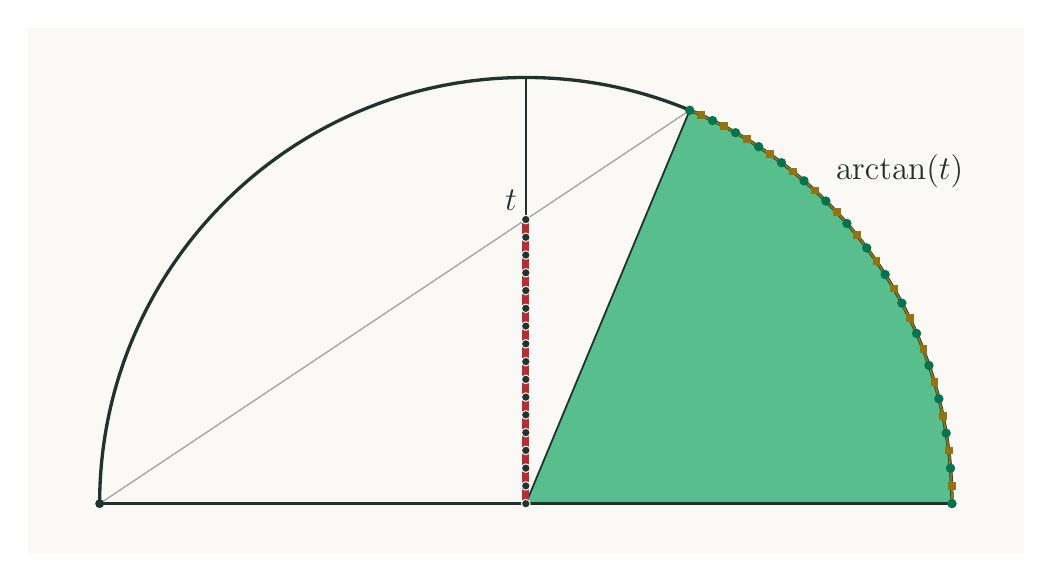
\begin{tikzpicture}[baseline=(current bounding box.north),x=1pt,y=1pt,line cap=round,line join=round]
\useasboundingbox (0,0) rectangle (360,190);
\definecolor{paper}{HTML}{FAF9F5}
\definecolor{semicircle}{HTML}{20332E}
\colorlet{lowerbound}{shared!85!semicircle}
\colorlet{upperbound}{yellow!59!semicircle}
\fill[paper] (0,0) rectangle (360,190);
\colorlet{lowerarea}{sharedfill}
\colorlet{upperarea}{overfill}
\colorlet{addition}{lowerbound!76!lowerarea}
\colorlet{cutoff}{yellow!85!upperarea}
\tikzset{chord/.style={lowerbound,line width=.65pt},tangent/.style={upperbound,line width=.65pt},chord trace/.style={chord,line width=1.25pt,dash pattern=on 5.5pt off 2.3pt},tangent trace/.style={tangent,line width=1.25pt,dash pattern=on 3.7pt off 2.2pt}}
\fill[upperarea] (180,18) -- (334,18) -- (334,24.4167) -- (332.9343,37.1834) -- (330.8247,49.7526) -- (327.7143,62) -- (323.6644,73.8121) -- (318.7525,85.0891) -- (313.068,95.7476) -- (306.7089,105.7215) -- (299.7778,114.963) -- (292.3784,123.4414) -- (284.6122,131.1429) -- (276.5763,138.0678) -- (268.3607,144.2295) -- (260.0475,149.6517) -- (251.7099,154.3664) -- (243.4118,158.4118) -- (239.2308,160.1538) -- cycle;
\fill[lowerarea] (180,18) -- (334,18) -- (333.4662,30.8111) -- (331.8759,43.4897) -- (329.2615,55.9077) -- (325.6757,67.9459) -- (321.188,79.4975) -- (315.8824,90.4706) -- (309.8528,100.7904) -- (303.2,110.4) -- (296.0274,119.2603) -- (288.4379,127.3491) -- (280.5308,134.66) -- (272.4,141.2) -- (264.1315,146.9879) -- (255.8031,152.0518) -- (247.4831,156.427) -- (239.2308,160.1538) -- cycle;
\draw[semicircle,line width=.85pt] (26,18) -- (334,18);
\draw[semicircle,line width=1.2pt] (334,18) arc[start angle=0,end angle=180,radius=154pt];
\draw[semicircle,line width=.65pt] (180,18) -- (239.2308,160.1538);
\draw[semicircle!42!paper,line width=.5pt] (26,18) -- (239.2308,160.1538);
\draw[chord] (334,18) -- (333.4662,30.8111) -- (331.8759,43.4897) -- (329.2615,55.9077) -- (325.6757,67.9459) -- (321.188,79.4975) -- (315.8824,90.4706) -- (309.8528,100.7904) -- (303.2,110.4) -- (296.0274,119.2603) -- (288.4379,127.3491) -- (280.5308,134.66) -- (272.4,141.2) -- (264.1315,146.9879) -- (255.8031,152.0518) -- (247.4831,156.427) -- (239.2308,160.1538);
\draw[tangent] (334,18) -- (334,24.4167) -- (332.9343,37.1834) -- (330.8247,49.7526) -- (327.7143,62) -- (323.6644,73.8121) -- (318.7525,85.0891) -- (313.068,95.7476) -- (306.7089,105.7215) -- (299.7778,114.963) -- (292.3784,123.4414) -- (284.6122,131.1429) -- (276.5763,138.0678) -- (268.3607,144.2295) -- (260.0475,149.6517) -- (251.7099,154.3664) -- (243.4118,158.4118) -- (239.2308,160.1538);
\fill[semicircle] (26,18) circle[radius=1.6pt];
\fill[lowerbound] (334,18) circle[radius=1.7pt];
\fill[lowerbound] (333.4662,30.8111) circle[radius=1.7pt];
\fill[lowerbound] (331.8759,43.4897) circle[radius=1.7pt];
\fill[lowerbound] (329.2615,55.9077) circle[radius=1.7pt];
\fill[lowerbound] (325.6757,67.9459) circle[radius=1.7pt];
\fill[lowerbound] (321.188,79.4975) circle[radius=1.7pt];
\fill[lowerbound] (315.8824,90.4706) circle[radius=1.7pt];
\fill[lowerbound] (309.8528,100.7904) circle[radius=1.7pt];
\fill[lowerbound] (303.2,110.4) circle[radius=1.7pt];
\fill[lowerbound] (296.0274,119.2603) circle[radius=1.7pt];
\fill[lowerbound] (288.4379,127.3491) circle[radius=1.7pt];
\fill[lowerbound] (280.5308,134.66) circle[radius=1.7pt];
\fill[lowerbound] (272.4,141.2) circle[radius=1.7pt];
\fill[lowerbound] (264.1315,146.9879) circle[radius=1.7pt];
\fill[lowerbound] (255.8031,152.0518) circle[radius=1.7pt];
\fill[lowerbound] (247.4831,156.427) circle[radius=1.7pt];
\fill[lowerbound] (239.2308,160.1538) circle[radius=1.7pt];
\fill[upperbound] (332.6,23.0167) rectangle (335.4,25.8167);
\fill[upperbound] (331.5343,35.7834) rectangle (334.3343,38.5834);
\fill[upperbound] (329.4247,48.3526) rectangle (332.2247,51.1526);
\fill[upperbound] (326.3143,60.6) rectangle (329.1143,63.4);
\fill[upperbound] (322.2644,72.4121) rectangle (325.0644,75.2121);
\fill[upperbound] (317.3525,83.6891) rectangle (320.1525,86.4891);
\fill[upperbound] (311.668,94.3476) rectangle (314.468,97.1476);
\fill[upperbound] (305.3089,104.3215) rectangle (308.1089,107.1215);
\fill[upperbound] (298.3778,113.563) rectangle (301.1778,116.363);
\fill[upperbound] (290.9784,122.0414) rectangle (293.7784,124.8414);
\fill[upperbound] (283.2122,129.7429) rectangle (286.0122,132.5429);
\fill[upperbound] (275.1763,136.6678) rectangle (277.9763,139.4678);
\fill[upperbound] (266.9607,142.8295) rectangle (269.7607,145.6295);
\fill[upperbound] (258.6475,148.2517) rectangle (261.4475,151.0517);
\fill[upperbound] (250.3099,152.9664) rectangle (253.1099,155.7664);
\fill[upperbound] (242.0118,157.0118) rectangle (244.8118,159.8118);
\definecolor{inputsegment}{HTML}{B52D34}
\draw[semicircle,line width=.65pt] (180,18) -- (180,172);
\draw[inputsegment,line width=2.4pt] (180,18) -- (180,120.6667);
\filldraw[fill=semicircle,draw=paper,line width=.35pt] (180,18) circle[radius=1.55pt];
\filldraw[fill=semicircle,draw=paper,line width=.35pt] (180,24.4167) circle[radius=1.55pt];
\filldraw[fill=semicircle,draw=paper,line width=.35pt] (180,30.8333) circle[radius=1.55pt];
\filldraw[fill=semicircle,draw=paper,line width=.35pt] (180,37.25) circle[radius=1.55pt];
\filldraw[fill=semicircle,draw=paper,line width=.35pt] (180,43.6667) circle[radius=1.55pt];
\filldraw[fill=semicircle,draw=paper,line width=.35pt] (180,50.0833) circle[radius=1.55pt];
\filldraw[fill=semicircle,draw=paper,line width=.35pt] (180,56.5) circle[radius=1.55pt];
\filldraw[fill=semicircle,draw=paper,line width=.35pt] (180,62.9167) circle[radius=1.55pt];
\filldraw[fill=semicircle,draw=paper,line width=.35pt] (180,69.3333) circle[radius=1.55pt];
\filldraw[fill=semicircle,draw=paper,line width=.35pt] (180,75.75) circle[radius=1.55pt];
\filldraw[fill=semicircle,draw=paper,line width=.35pt] (180,82.1667) circle[radius=1.55pt];
\filldraw[fill=semicircle,draw=paper,line width=.35pt] (180,88.5833) circle[radius=1.55pt];
\filldraw[fill=semicircle,draw=paper,line width=.35pt] (180,95) circle[radius=1.55pt];
\filldraw[fill=semicircle,draw=paper,line width=.35pt] (180,101.4167) circle[radius=1.55pt];
\filldraw[fill=semicircle,draw=paper,line width=.35pt] (180,107.8333) circle[radius=1.55pt];
\filldraw[fill=semicircle,draw=paper,line width=.35pt] (180,114.25) circle[radius=1.55pt];
\filldraw[fill=semicircle,draw=paper,line width=.35pt] (180,120.6667) circle[radius=1.55pt];
\node[anchor=south east,inner sep=1pt,text=semicircle,font=\large] at (178,122.6667) {\(t\)};
\node[anchor=west,inner sep=1pt,text=semicircle,font=\large] at (290.88,138.12) {\(\arctan(t)\)};
\end{tikzpicture}
\end{document}
